
\section{Evaluation}
\label{sec:evaluation}

We implemented our technique in an open-source programming tool.
Our tool employs WEKA \cite{Hall:2009} to implement the PART learning algorithm
 to extract rules, and uses MySQL~\cite{mysql} as the backend database engine
to check the validity of each output query.
When a SQL query is synthesized,
our tool executes the synthesized query on the backend database,
and checks whether the output query result matches the given example output.

We next describe the evaluation of our prototype tool.

\subsection{Research Questions}

We aim to investigate the following research questions:

\begin{itemize}
\item Is the supported SQL subset expressive enough to describe
queries that real end-users require?

\item Can our technique efficiently find a SQL query
from small input-output examples?

%\item Does the inferred SQL query correctly express end-users'
%intention and produce the expected output? If not, how many
%additional examples does a user need to provide before our
%approach infers a correctly-behaved SQL query?

\end{itemize}


\subsection{SQL Query Synthesis Scenarios}

To answer these two questions, we collected a set
of SQL query synthesis scenarios in the following
two ways. First, we picked
up 6 SQL exercises from a classic database textbook~\cite{cowbook}.
Those 6 SQL exercises cover many commonly-used SQL features,
which a database course instructor think would be the most useful parts,
and expect her students to get familiar with. Second, we collected
5 SQL problems raised by real end-users from popular online help forums
~\cite{stackoverflow, tutorialized, dbjournal}.

%evaluation
%subjects from two major sources: exercises from classic
%database textbooks like, and real-world questions
%that end-user asked on well-known online help forums. Specifically,
%we aim to apply our implemented tool solve SQL query related questions
%after Chapter 3 (SQL DML) in~\cite{cowbook}. We have also collected
%19 end-user questions from online forums, and plan to apply our
%tool to solve them.

For a given exercise or problem, if it
has already been associated with input-output examples (e.g.,
those provided by users from online forums),
we directly apply our tool on the existing examples.
Otherwise, we manually provide small concise and representative
input-output examples for our tool.
If for a given exercise or problem, our tool inferred
a SQL query that does not behave as we expected when applied
to other inputs, we will manually find an input on which the
SQL query misbehaves and reapplied our tool to the new input. We
repeat this process until our tool infers a desirable SQL query.

\subsection{Experimental Results}

\begin{table}[t]
\setlength{\tabcolsep}{.14\tabcolsep}
\begin{tabular}{|c|c|c|c|c|}
\hline
 & \#Total& \#Solved& Time Cost (s) & Human Effort (m)\\
 \hline
 Textbook exercises &  6 &  5 &  30 & 3 \\
\hline
 Forum problems &  5 &  5  &  60 & 5\\
\hline
\end{tabular}

\Caption{{\label{tab:results} Experimental results of synthesizing
SQL queries for 6 exercises from a classic database textbook~\cite{cowbook},
and 5 real problems from online forums. Column `\#Total' is the total
number of exercises or problems used in the experiments. Column
`\#Solved' is the number of solved
exercises or problems by our technique. Column `Time Cost(s)'
records the average time (in seconds) used to solve each exercise or problem.
Column `Human Effort(m)' is the average time (in minutes) spent in
preparing input-output examples for each exercise or problem without
existing examples.}}
\end{table}

For each SQL synthesis scenario, we measured two results.
The time cost in producing
a desirable SQL query by our tool, and
the time we spent in writing input-output examples.
%For each exercise or problem, we also record
%how much time we spent in writing input-output examples.
Table~\ref{tab:results} summarizes our experimental results.

As shown in Table~\ref{tab:results}, our technique synthesized
expected SQL queries for 10 out of 11 scenarios
within a very small amount of time (less than 1 minute each).
The human effort spent in providing input-output examples
is also very limited: it took us less than 5 minutes for one scenario.
%per exercise (or problem).


\subsubsection{A Real Example}


\begin{figure*}[t]
  \centering
  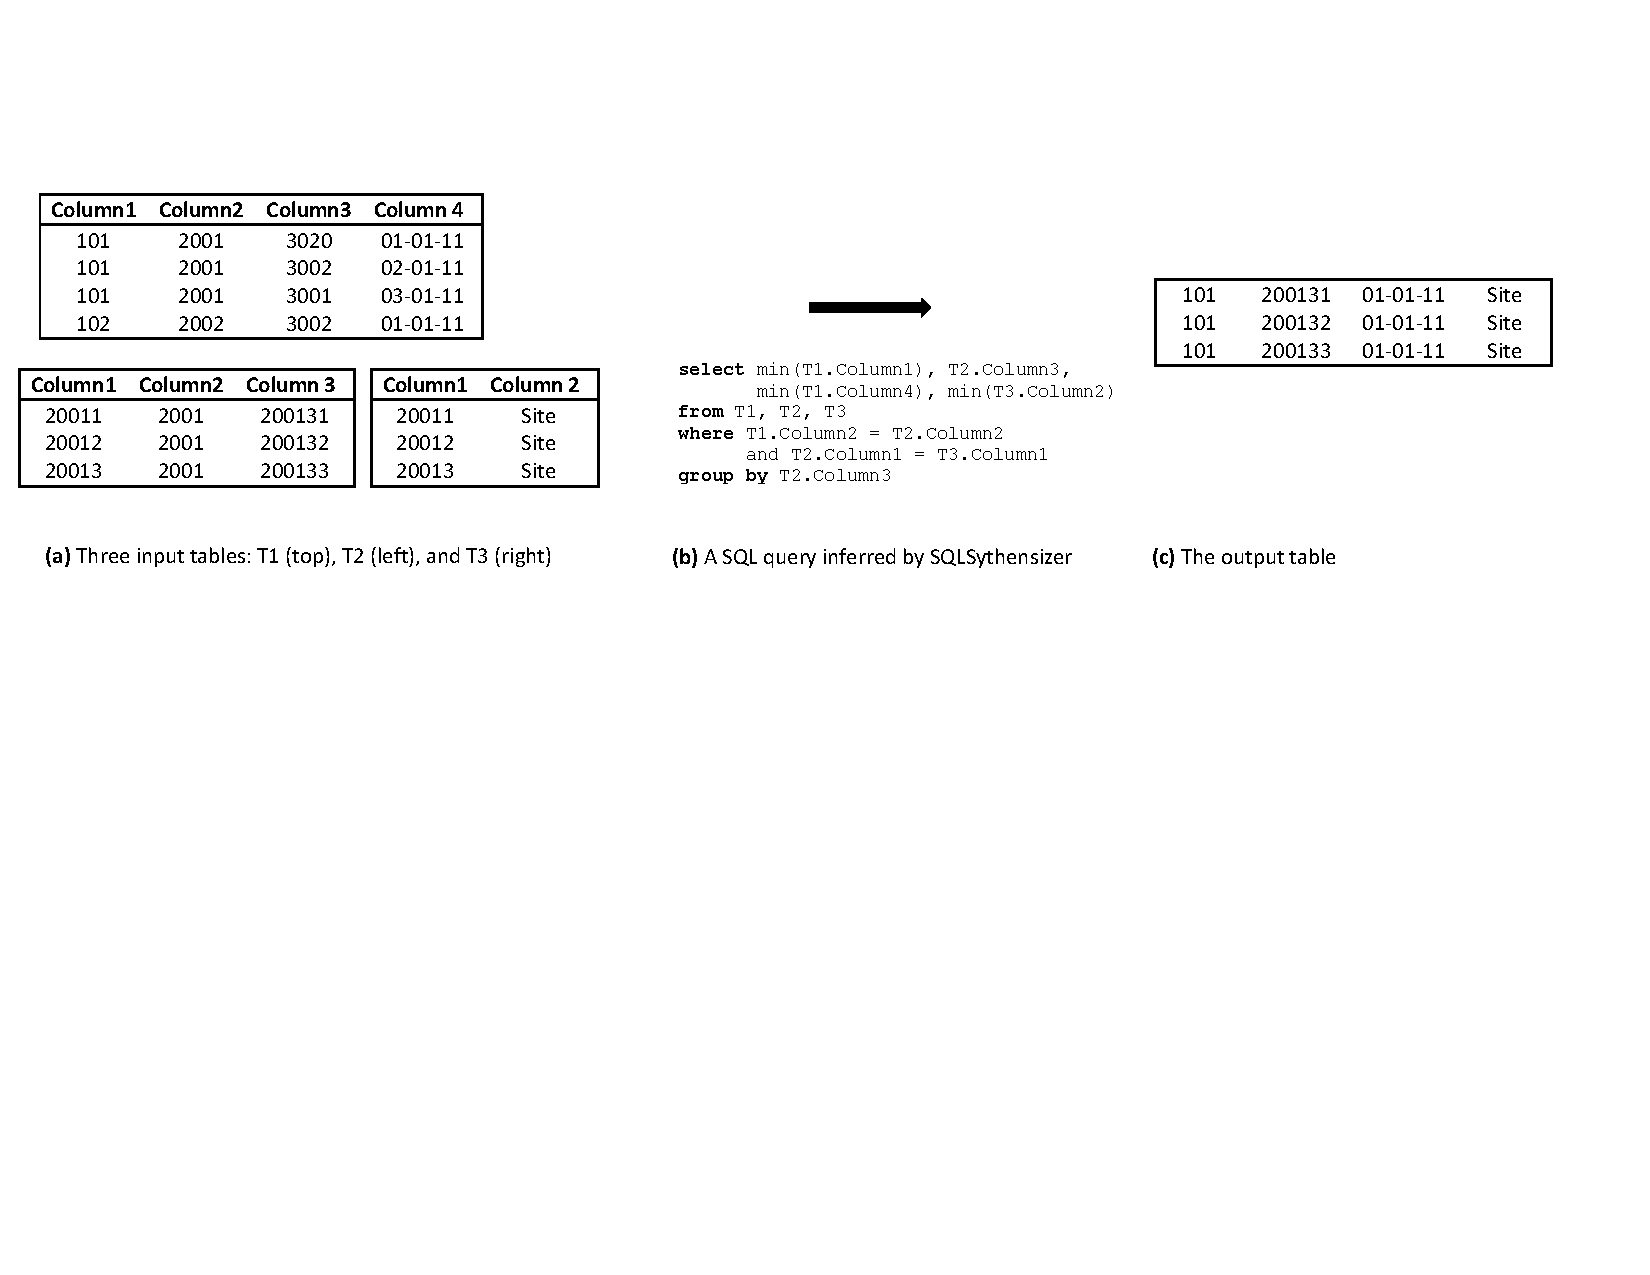
\includegraphics[scale=0.70]{example2}
  \vspace*{-1.0ex}\caption {{\label{fig:example2} Input-output
  examples ((a) and (c)) taken from an online SQL help forum
  thread. \ourtool automatically sythensizes 6 SQL queries that
  can produce the output table from the three input tables.
  (b) shows the highest ranked SQL query.
}}
\end{figure*}

We use a real SQL question from
an online forum\footnote{\url{http://forums.tutorialized.com/sql-basics-113/join-problem-147856.html}} to illustrate
\ourtool's effectiveness.
The question was started by a novice user, who needed help to write a
SQL query to get result from three input tables. In this question, the
novice user described his required query in a few paragraphs of
English, but also include several small, representative input-output
examples as shown in Figure~\ref{fig:example2}, to better express
his intention. 
This question receives no replies as of April 2013 and we speculated that
writing a SQL query to join three tables to produce certain output results
is non-trivial.

We ran \ourtool on the input-output examples
in Figure~\ref{fig:example2}. The tool produced 6 valid answers
in less than 1 minutes, all of which satisfy the given examples. The
highest ranked SQL query is shown in Figure~\ref{fig:example2},
which is quite unintuitive to write. The SQL query in
Figure~\ref{fig:example2}
first joins three input tables
on columns \CodeIn{T1.Column2}, \CodeIn{T2.Column2},
\CodeIn{T2.Column1}, and \CodeIn{T3.Column1} using some
selected columns, and then aggregates the results based on
column \CodeIn{Table2.Column3}'s value. Finally, it
returns the minimal values of columns \CodeIn{T1.Column1}, \CodeIn{T1.Column4}, and \CodeIn{T3.Column2}
from each aggregated group as the results.




\subsection{Experimental Conclusions}

Our initial experimental results are promising.
It shows that the supported SQL subset is
expressive enough to describe a variety of useful database queries.
It also demonstrates the usefulness of our SQL query
synthesis technique.  In particular, our SQL query synthesis technique only requires a small amount of
human effort and small input-output examples. It infers 
desirable SQL queries on both database textbook exercises
and online forum problems, even solving problems that receive no reply
from popular online forums.




